\documentclass[twocolumn,10pt]{article}


\usepackage{times}
\usepackage{cite}
\usepackage{multirow}
\usepackage[tight,footnotesize]{subfigure}
%\usepackage{subfig}
\usepackage{listings}
\usepackage{url}
\usepackage{xspace}
\usepackage{amsmath}
\usepackage{amsfonts}
\usepackage{amssymb}
\usepackage{graphicx}
\newcommand{\comment}[1]{}
\newcommand{\eat}[1]{}
\usepackage{booktabs, lastpage}
\usepackage{tikz}
\usetikzlibrary{positioning}
\usepackage{mdframed, fancyvrb}
\usepackage[scaled]{beramono}
\usepackage{rotating}
\definecolor{boxcolor}{gray}{0.9}
\newmdenv[linecolor=boxcolor, backgroundcolor=boxcolor, skipabove=\parsep, skipbelow=\parsep, innerleftmargin=2pt, innerrightmargin=2pt]{codeblock}
\newcommand{\myparait}[1]{\smallskip\noindent{\em {#1}:}~}
\newcommand{\myparaq}[1]{\medskip\noindent{\bf {#1}?}~}
\newcommand{\mypara}[1]{\medskip\noindent{\bf {#1}:}~}
\newcommand{\myparatight}[1]{\smallskip\noindent{\bf {#1}:}~}

\newcounter{packednmbr}
\newenvironment{packedenumerate}{\begin{list}{\thepackednmbr.}{\usecounter{packednmbr}\setlength{\itemsep}{1pt}\addtolength{\labelwidth}{-5pt}\setlength{\leftmargin}{\labelwidth}\setlength{\listparindent}{\parindent}\setlength{\parsep}{1pt}\setlength{\topsep}{3pt}}}{\end{list}}
\newenvironment{packeditemize}{\begin{list}{$\bullet$}{\setlength{\itemsep}{1pt}\addtolength{\labelwidth}{-5pt}\setlength{\leftmargin}{\labelwidth}\setlength{\listparindent}{\parindent}\setlength{\parsep}{1pt}\setlength{\topsep}{3pt}}}{\end{list}}
\usepackage{shortcuts}
\usepackage{hyperref}
\hypersetup{
  colorlinks=true,      % false: boxed links; true: colored links
  linkcolor=blue,       % color of internal links
  citecolor=magenta,    % color of links to bibliography
  filecolor=cyan,       % color of file links
  urlcolor=red          % color of external links
}

\definecolor{shadecolor}{gray}{0.9}

\frenchspacing
\pagestyle{plain}

\def\ala{{\`{a} la}~}
\def\ie{{i.e.}}
\def\eg{{e.g.}}
\def\etal{{et al.}~}
\def\wrt{{w.r.t.}~}
\def\viz{viz.~}
\def\vs{vs.~}
\def\etc{etc.}

\definecolor{codegreen}{rgb}{0,0.6,0}
\definecolor{codegray}{rgb}{0.5,0.5,0.5}
\definecolor{codepurple}{rgb}{0.58,0,0.82}
\definecolor{backcolour}{rgb}{0.95,0.95,0.92}

\begin{document}
\title{18731 Spring 2022 Project Final Report\\
  Security Policy Modeling For Web Applications}

\author{
  Rongjian Xiao \\ rongjiax@andrew.cmu.edu \and
  Peiyuan Shen \\ peiyuans@andrew.cmu.edu \and
  Sicheng Mao \\ sichengm@andrew.cmu.edu \and
  Qingxuan Kuang \\ qkuang@andrew.cmu.edu
}

\maketitle

\begin{abstract}
  % Quick 4-5 sentence abstract of the work: 1. Motivate problem 2. What is
  % known 3. What you propose to do that is different 4. Expected outcomes

  % Motivate problem
  Analyzing security policies is important for access management of web
  applications.
  % What is known
  Many web frameworks provide Domain-Specific Languages (DSLs) to specify
  security policies for APIs.
  %
  However, many security policies are often not specific or missing.
  % What you propose to do that is different
  This project proposed a DSL to describe the security policies of analyzed
  systems and perform a taint analysis on a target web application system to
  synthesize the security policies.
  % Expected outcomes
  Given the security policies we synthesized, developers can easily identify
  potential vulnerabilities of the target system and improve development
  efficiency.

\end{abstract}

\section{Introduction}% (1 page}


%   \item Para 1 what is the broad problem space you are working on
%   \item Para 2 what is the sub problem you are working on
% What is the problem that this project is going to address?
Access management for web applications is a critical component for web
applications.
% Does it matter: why is the problem important?
Many web frameworks provide DSLs to specify security policies for APIs, but
developers still mix the access control of the data with other application
logic.
% Who will benefit when the problem is solved
Although many applications provide official documents for developers,
permission control is often not specific or even missing.
%
Therefore, the goal of this project is to extract a relatively comprehensive
list of security policies for developers to reason about.

%   \item Para 3 what is known from the prior work
%   \item Para 4 What are the shortcomings of prior work

%   \item Para 5 What is your works contribution
%   \item Para 6 what are the main ideas/approaches you are taking
%   \item Para 7 what has been implemented
%   \item Para 8 what are some of the key outcomes/performance results
In this project we present a security policy synthesizer

% We separate the whole project to 4 parts below.
% \begin{enumerate}
%   \item Identify security-sensitive events. We consider all operations that may
%         affect the integrity of database to be security-sensitive events
%         (queries that insert, delete, or update the database).

%   \item Construct calling-context topology. For each security-sensitive event e,
%         builds a topo graph of contexts who start from e and end at program
%         entry points.

%   \item Generate security policies. For each API,  get the call-chain paths for
%         all function calls involve security-sensitive events

%   \item Detect Potential Vulnerabilities. Through the policies automatically
%         generated by the program, the existing security risks are manually
%         identified
% \end{enumerate}

% From the prior work, We have used doop to taint analysis the lancie api, and got
% the corresponding analysis file (such as CallGraphEdge.csv).

% Although we have obtained this result, doop itself has compatibility problems
% (not compatible with Mac OS), which we cannot solve.

In this project we are using lancie api~\footnote{Publicly available at:
  \url{https://github.com/AreaFiftyLAN/lancie-api.}} for analysis use case.
%
Through the analysis of lancie api, we design a simple modeling language below
that describes security policies.
% \begin{itemize}
%   \item Policy $\rightarrow$ Statement
%   \item Principal $\rightarrow$ (Role $|$ Role(Condition) $|$ IsAuthenticated)
%         \begin{itemize}
%           \item[*] Role $\rightarrow$ ROLE\_ADMIN $|$ ROLE\_OPERATOR $|$ ROLE\_COMMITTEE $|$ ROLE\_USER
%           \item[*] Condition $\rightarrow$ string$*$
%         \end{itemize}
%   \item Action $\rightarrow$ string$*$
%   \item Resource $\rightarrow$ string$*$
% \end{itemize}

We have written a program that scans the lancie api project file, identifies
security-sensitive events, and automatically generates corresponding
policies (Figure \ref{fig:policies}) based on these Identify security-sensitive
events and call graph. Then we detected Potential Vulnerabilities based on these
policies.
% \begin{figure}[htp]
%   \centering
%   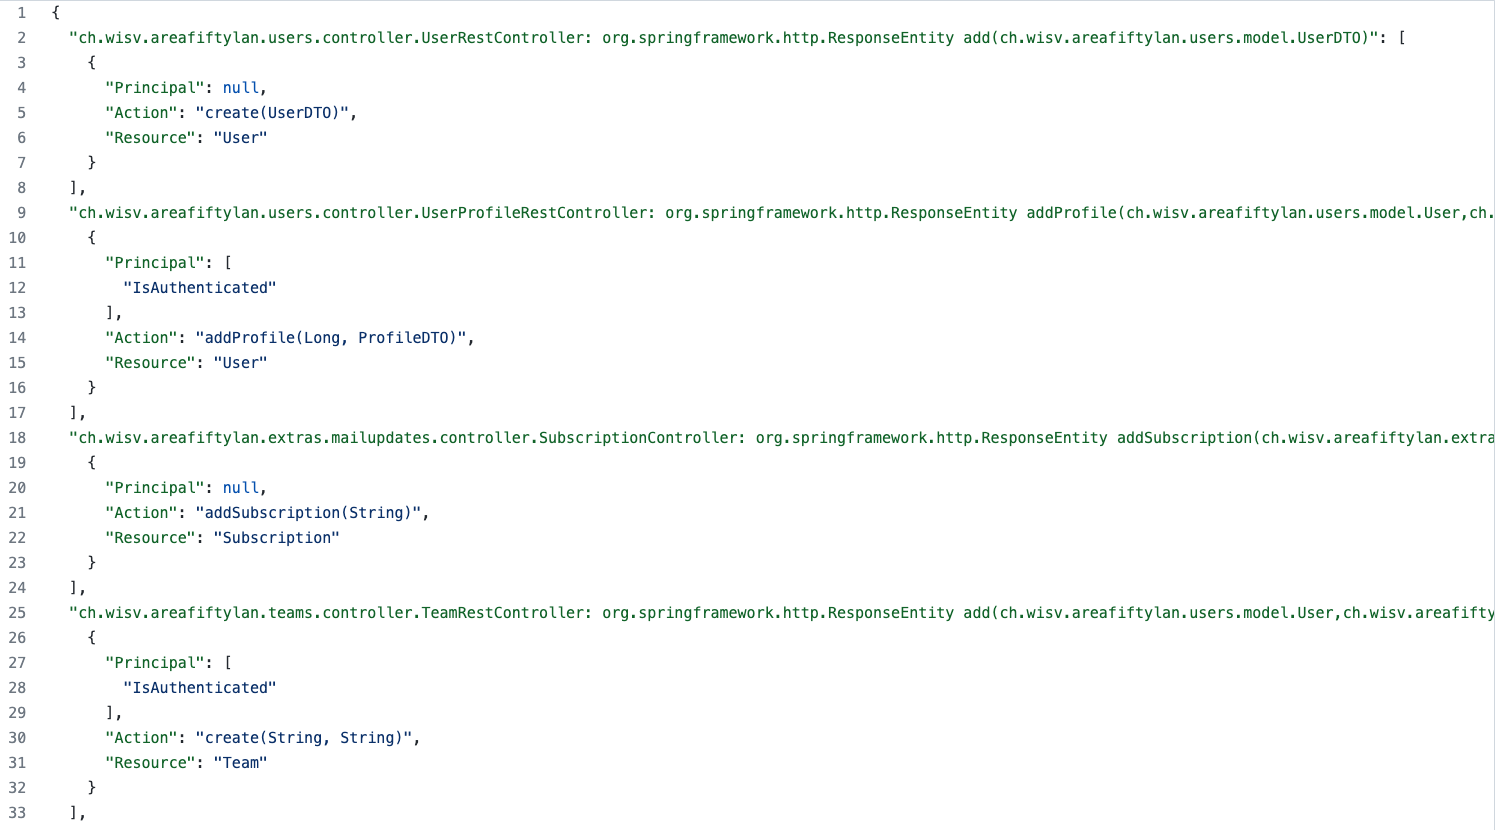
\includegraphics[width=0.45\textwidth]{img/policies.png}
%   \caption{polices}
%   \label{fig:policies}
% \end{figure}


\section{Background and Related Work} %1 page
% what’s proposed already? What have others done already? What did they learn?
% taxonomies prior work and highlight what is new/different in your work vs
% theirs
In this section, we give an overview of one of the most popular web application
framework, Spring~\cite{spring+security:home}, and review prior work related to
our projects.

\subsection{Spring}

Spring~\cite{spring+security:home} is said to be the most popular Java web
application framework.
%
The Spring Framework is an application framework and inversion of control
container for the Java platform.
%
Spring Security~\cite{spring+security:method} is a powerful authentication and
access-control framework, which is the standard for securing Spring-based
applications.
%
Spring security provides comprehensive and extensible support for both
authentication and authorization, and prevents attacks like session fixation,
clickjacking, etc.

\subsection{Java Program Analysis}

An access control policy is an expressive specification of what resources can be
accessed, by whom, and under what conditions.
%
Bakers \etal~\cite{Backes+etal:2018:Zelkova} presents a formalization of the
Amazon Web Services (AWS) policy language  that lets users govern access to AWS
resources. This paper also presents an analysis tool, ZELKOVA, for verifying
policy properties.

Static information-flow analysis (especially taint-analysis) is a key technique
to compute where sensitive or untrusted data can propagate in a program.
Points-to analysis~\cite{10.1145/3133926} is a fundamental static program
analysis, computing what abstract objects a program expression may point to.

Bravenboer \etal~\cite{Bravenboer:2009:Doop} presented Doop\footnote{Publicly
  available at: \url{http://doop.program-analysis.srg/}.} which is a framework
for Java pointer and taint analysis.
%
Doop specifies pointer analysis algorithms declaratively using Datalog: a
logic-based language for defining recursive relations.
%
At its core, Doop is a collection of various analyses expressed in the form of
Datalog rules.

Antoniadis \etal~\cite{Antoniadis+etal:2020:Java} proposed a static
analysis framework called JackEE for Java Application, and introduced a
sound-modulo-analysis model of Java HashMap to improve precision and
scalability. JackEE can analyze both Servlets and Spring APIs. JackEE is also
evaluated through realistic benchmarks. It is proved to have a higher
reachability than some other popular tools like Doop.

Tripp \etal~\cite{10.1145/1542476.1542486} designed a static Taint Analysis for
Java (TAJ) that can analyze applications of any size, especially industry-length
programs. TAJ has the techniques to handle reflective calls, flow through
containers, nested taint, and issues in generating useful reports.

Lerch \etal~\cite{10.1145/2635868.2635878} presented FlowTwist, a taint-analysis
approach that works inside-out. They expose a design of the analysis approach
based on the IFDS algorithm and several extensions to IFDS that enable reporting
of error situations to security analysts.

Sridharan \etal~\cite{10.1145/2076021.2048145} added framework-for-framework
support to a state-of-the-art taint-analysis engine, which is useful for web
applications that utilize one or more web frameworks.

Mues \etal~\cite{10.1007/978-3-030-63461-2_7} presented JAINT, a generic security
analysis for JAVA Web-applications in which dynamic taint analysis is
integrated. They also design a domain-specific language for users to specify
taint-based security analyses for applications.

Rather than taking a specification of this logic as input, RoleCast
\etal~\cite{10.1145/2048066.2048146} is a system that statically identifying
security logic that mediates security-sensitive events in Web applications. It
identifies security-critical variables and applies role-specific variable
consistency analysis to find missing security checks. RoleCast performs well for
PHP and JSP applications.

Arzt \etal~\cite{10.1145/2594291.2594299} presented FlowDroid, a static taint
analysis for Android applications, which makes use of Android's precise
lifecycle to handle callbacks, and context, flow, field and object-sensitivity
to minimize faults. They proposed DroidBench, for Android applications
taint-analysis evaluation.

Yang \etal~\cite{6394931} proposed an approach called
Leak Miner for detecting information leakage on Android applications on market
site before users download them, which avoids runtime overhead to normal usage.

Pauck \etal~\cite{10.1145/3236024.3236029} presented ReproDroid, a framework
allowing the accurate comparison of Android taint analysis tools, inferring the
ground truth for data leaks in apps, in automatically applying tools to
benchmarks, and in evaluating the obtained results.

Ujcich \etal~\cite{Ujcich+etal:2020:EventScope} in 2020 proposed a technique
called EventScope to extend the vulnerability identification~\cite{6994333} to
SDN. EventScope automatically analyzes SDN control plane event usage, discovers
candidate vulnerabilities based on missing event-handling routines, and
validates vulnerabilities based on data plane effects.


\section{Design}% 1-2pg}
% What are plausible alternatives you considered?

% provide block diagrams of how the system works, what are the interfaces between
% components

% what are the key ideas and technical challenges

% how did you implement/prototype said ideas
\begin{figure}[tbp]
  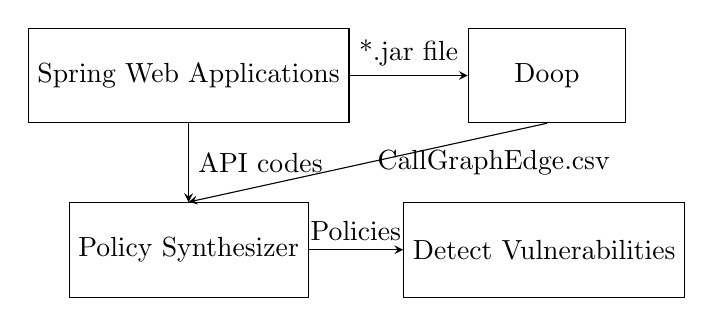
\begin{tikzpicture}

    \node [draw,
      minimum width=2cm,
      minimum height=1.2cm,
    ]  (app) {Spring Web Applications};

    \node [draw,
      minimum width=2cm,
      minimum height=1.2cm,
      right=1.5cm of app,
    ]  (doop) {Doop};

    \node [draw,
      minimum width=2cm,
      minimum height=1.2cm,
      below=1cm of app,
    ]  (syn) {Policy Synthesizer};

    \node [draw,
      minimum width=2cm,
      minimum height=1.2cm,
      right=1.2cm of syn,
    ]  (detect) {Detect Vulnerabilities};

    \draw[-stealth] (app.east) -- (doop.west)
    node[midway,above]{*.jar file};

    \draw[-stealth] (app.south) -- (syn.north)
    node[midway,right]{API codes};

    \draw[-stealth] (doop.south) -- (syn.north)
    node[midway,right]{CallGraphEdge.csv};

    \draw[-stealth] (syn.east) -- (detect.west)
    node[midway,above]{Policies};

  \end{tikzpicture}
  \caption{System block diagram.}
  \label{fig:desgin}
\end{figure}

\subsection{Overview}

\subsection{Policy Synthesizer}

\subsubsection{Identify security-sensitive events}
\subsubsection{Construct calling-context topology}
\subsubsection{Generate security policies}

\section{Evaluation}% 1-2pgs}

% what is your evaluation setup? methodology? metrics of interest?

% What did you do  test out the hypotheses? (E.g.
% measurements, simulations, constructing code)


% What are the key results .
In this section, we discuss our implementation of the system and evaluate the
security policies generated by our policy synthesizer.

\subsection{Implementation}
Our system choose \lancie as the target spring application to evaluate.
%
As of May 1st, \lancie contains $10498$ lines of java codes.
%
\lancie clearly separated APIs and functions with database manipulation, making
it an ideal target for us to evaluate.
%
We installed Doop on a Ubuntu 20.04 LTS image and used it to perform taint
analysis on \lancie and got the \textit{CallGraphEdge.csv} file which contains
$57925$ lines.

We implemented our policy synthesizer in Python and the synthesizer consists of
$214$ lines of codes as shown in Appendix.
%
We automatically synthesized policies for $67$ APIs.
%
Of all $67$ policies we generated, only three of them contain two statements and
all the other policies contain one statement.
%
We manually checked all $67$ policies to make sure that the synthesized output
is as expected.

\subsection{Vulnerabilities Detection}
Most software has the need to use and modify the database, but different roles
should have different permissions to operate the database. Once there is a role
in operating the database incorrectly, it will cause a lot of losses to the
enterprise. However, when software engineers develop software, it is possible to
forget to check permissions, which leads to some Vulnerabilities. Therefore,
from our generated policies, we can easily observe what vulnerabilities are in
the software.

\onecolumn
\begin{sidewaysfigure}[p]
  \caption{Manually detected vulnerabilities in LANcie API.}
  \label{tab:api}
  \centering
  \begin{tabular}{ |p{0.15\columnwidth} | p{0.15\columnwidth} | p{0.3\columnwidth} | p{0.2\columnwidth}|}
    \hline
    File                                                                         & Function & Policy & Vulnerabilities \\
    \hline
    ch.wisv.areafiftylan. users.controller. UserRestController                   &
    org.springframework. http.ResponseEntity add(UserDTO)                        &
    \begin{lstlisting}
"Principal": null,
"Action": "create(UserDTO)",
"Resource": "User"
    \end{lstlisting}                                                       &
    Modify the database without checking the role                                                                      \\
    \hline

    \hline
    ch.wisv.areafiftylan. extras.mailupdates. controller. SubscriptionController &
    org.springframework. http.ResponseEntity addSubscription (SubscriptionDTO)   &
    \begin{lstlisting}
"Principal": null,
"Action": "addSubscription",
"Resource": "Subscription"
    \end{lstlisting}                                                       &
    Modify the database without checking the role                                                                      \\
    \hline

    \hline
    ch.wisv.areafiftylan. products.controller. OrderRestController               &
    org.springframework. http.ResponseEntity createOrder (TicketDTO)             &
    \begin{lstlisting}
"Principal": null,
"Action": "create",
"Resource": "Order"
    \end{lstlisting}                                                       &
    Modify the database without checking the role                                                                      \\
    \hline

    \hline
    ch.wisv. areafiftylan.web. sponsor. controller. SponsorController            &
    org.springframework. http.ResponseEntity  createSponsor (Sponsor)            &
    \begin{lstlisting}
"Principal":[ROLE_COMMITTEE],
"Action": "createSponsor",
"Resource": "Sponsor"
    \end{lstlisting}                                                       &
    The administrator should also have the right to operate                                                            \\
    \hline
  \end{tabular}
\end{sidewaysfigure}
\twocolumn


\section{Conclusions and Limitations}% 0.25-0.5 pg}

 {
  \footnotesize
  \raggedright
  \bibliographystyle{abbrv}
  \bibliography{bib}
 }

\newpage
\onecolumn
\section{Appendix - Code}
\lstdefinestyle{mystyle}{
  backgroundcolor=\color{backcolour},
  commentstyle=\color{codegreen},
  keywordstyle=\color{magenta},
  numberstyle=\tiny\color{codegray},
  stringstyle=\color{codepurple},
  basicstyle=\ttfamily\footnotesize,
  breakatwhitespace=false,
  breaklines=true,
  captionpos=b,
  keepspaces=true,
  numbers=left,
  numbersep=5pt,
  showspaces=false,
  showstringspaces=false,
  showtabs=false,
  tabsize=2
}

\lstset{style=mystyle}
\subsection*{\centering \large genPolicy.py}
\lstinputlisting[label={lst:diffs}, language=Python]{genPolicy.py}

\end{document}

